%===============================================================================
% Autoři: Michal Bidlo, Bohuslav Křena, Jaroslav Dytrych, Petr Veigend a Adam Herout 2018
\chapter{Úvod}
Rozmach webových aplikácií priniesol prenos veľkého množstva dát medzi rôznymi systémami. Vymieňané dáta sú obvykle štrukturované a serializované v určenom formáte. Pri testovaní takýchto systémov vzniká problém získania testovacích dát, ktoré sú zvyčajne komplexné a je problematické vytvárať ich manuálne. Analýza týchto dát je zložitá a ťažko sa o nich vytvára celkový obraz pokiaľ nieje dostupná ich detailná špecifikácia. 

Cieľom tejto práce je vytvoriť nástroj pre analýzu stromových štruktúr z reálnych dát. Výsledkom analýzy je charakteristika dát, ktorá slúži na automatizovanú syntézu dát pre účely testovania. Dôraz kladie na zachovanie konkrétnych štruktúr a sémantiky ich hodnôt. Rovnako umožňuje verifikáciu vzorky dát voči vopred spracovaným dátam. 

Vytvorený nástroj je súčasťou platformy Testos \ref{Testos}, čo je projekt s cieľom vytvorenia sady nástrojov podporujúce automatizované testovanie. Nástroj aktívne využíva nástroje platformy pre detekciu sémantiky hodnôt a generovanie dát.   

Kapitola \ref{testing} predstavuje teoretické základy testovania softvéru, pričom sa zameriava na testovanie na dátach. Nasledujúca kapitola \ref{struktury} sa zaoberá štrukturovanými dátami a nástrojom, z ktorého táto práca vychádza. Kapitola \ref{navrh} rozoberá požiadavky na vytváraný nástroj a popisuje návrh architektúry a algoritmu. V poslednej kapitole \ref{zaver} sú zhrnuté doterajšie výsledky práce.   

     


\chapter{Testovanie softwaru}
\label{testing}
Testovanie softvéru je súbor procesov analyzujúcich softvér za účelom vyhodnotenia jeho vlastností a detekcie rozdielov medzi aktuálnym a požadovaným stavom \cite{Standard}. Táto kapitola najskôr predstavuje základné úrovne a druhy testovania. Následne popisuje testovanie založené na dátach a s tým spojenú rozhodovaciu tabuľku. Rozoberá spôsoby tvorby a voľby dát rozhodovacej tabuľky. V závere predstavuje platformu Testos.   

\bigskip
\section{Úrovne testovania}
Testy sú vytvárané na základe špecifikácií a požiadaviek dizajnových artefaktov alebo zdrojového kódu. Rôzne úrovne testovania sprevádzajú rozdielne vývojárske aktivity \cite{Ist}.
\subsection*{Jednotkové testovanie}
Jednotkové testovanie je zamerané na jednotky, predstavujúce najmenšie testovateľné komponenty testovaného systému. Zmyslom jednotkového testovania je validácia správania jednotky voči jej dizajnu. Zameriava sa na chyby na najnižšej úrovni. Testy vytvárajú samotný programátori počas vývoja.    
\subsection*{Integračné testovanie}
Integračné testovanie je cielené na korektnú komunikáciu medzi rozhraniami jednotiek, ktoré sú pre tento účel zlučované do podsystémov. Úlohou integračného testovania nie je nájdenie chýb v jednotlivých integrovaných jednotkách, ale overenie ich korektných integrácií. Predpokladá sa, že tieto chyby boli eliminované pri jednotkovom testovaní. Odhaľuje chyby v rozhraniach a stavoch jednotiek. Pri väčšom množstve rozhraní je vhodné zvoliť špecifický prístup k integračným testom. Obvyklé stratégie sú zdola nahor, zhora nadol, funkcionálna integrácia a veľký tresk \cite{Gst}. Zvyčajne ich tvoria vývojári alebo testeri v rámci tímu.
\subsection*{Systémové testovanie}
Systémové testovanie je zamerané na nájdenie chýb vo vlastnostiach plne integrovaného systému. Testovaný systém je tvorený komponentami, ktoré už úspešne prešli integračnými testami. Cieľom je detekcia nekonzistentností medzi týmito komponentami a systému ako celku voči špecifikácií požiadavkov. Systémové testovanie vykonáva oddelená skupina testerov mimo vývojového tímu. 
\subsection*{Akceptačné testovanie}
Akceptačné testovanie je proces s účelom overenia softvéru voči počiatočným stanoveným požiadavkám zákazníka a jeho aktuálnych potrieb. Často sa na ich vytváraní podieľa expert na doménu, pre ktorý sa softvér vyvíja. Zvyčajne je vytvorený zákazníkom alebo koncovým užívateľom a overuje, či dané riešenie pre užívateľa funguje \cite{Ast}.  

\section{Dynamické testovanie}
\label{Dyn_t}
Existuje mnoho prístupov k testovaniu softvéru. Na najvyššej úrovni sa testovanie rozdeľuje na {\it statické} a {\it dynamické} \cite{Ist}. Techniky, ktoré analyzujú a skúmajú program bez nutnosti jeho spustenia za účelom verifikácie,  spadajú do skupiny statického testovania. Zahrňuje posudzovanie dokumentov, kódu a jeho statickú analýzu (základná statická analýza zvyčajne prebieha na úrovni kompilátorov). Druhá skupina techník spadá do skupiny dynamického testovania, ktorá je zameraná na analýzu dynamického správania kódu s cieľom jeho validácie. Podmienkou použitia je úspešná kompilácia a spustenie kódu. Zahrňuje prácu so softvérom, kedy pre špecifické vstupy overuje a analyzuje správnosť výstupov.

Dynamické testovanie môže byť ďalej rozdelené na {\it funkcionárne} a {\it nefukncionárne}. Kým funkcionárne testovanie adresuje splnenie požiadaviek, nefukcionárne je mierené na ostatné oblasti ako bezpečnosť, výkonnosť, použiteľnosť, správa pamäti a iné. Podľa znalosti kódu sa delí na {\it black-box, white-box a grey-box} testovanie.

Diplomová práca sa zameriava na testovanie založené na dátach, ktoré vychádza z funkcionálneho black-box testovania, ale výsledný nástroj môže byť prínosný aj pre iné prístupy.


\subsection*{Black-box testovanie}
{\it Black-box testovanie} (tiež známe ako {\it testovanie založené na dátach}) zoskupuje techniky tvorby testovacích prípadov na základe špecifikácií podľa analýzylpopisu softvéru bez znalosti jeho vnútornej štruktúry  \cite{Ast}. Ich hlavným zameraním je odhalenie okolností, pri ktorých sa systém správa odlišne od špecifikácií.  Testovacie dáta závisia na popise očakávaní od testovaného softvéru, napríklad vo forme manuálu či popisu procesu.

Black-box testovanie môže byť použité na všetkých úrovniach testovania. Pre nižšie úrovne jednotkového a integračného testovania sa dá použiť ako počiatočný bod pre tvorbu testov na základe dizajnu alebo aj požiadaviek. Veľmi užitočné sú na vyšších úrovniach (systémová a akceptačná), kde sú testy založené na požiadavkách  \cite{Gst}.

\subsection*{White-box testovanie}
Techniky white-box testovania vytvárajú testovacie prípady podľa vnútornej štruktúry komponentu alebo systému. Hlavný dôraz kladú na vetvy, jednotlivé podmienky a výrazy tradične v zdrojovom kóde. Primárne sa využívajú v jednotkovom a integračnom testovaní. Všetky testovacie techniky tohoto druhu od testera vyžadujú znalosť danej štruktúry, teda programovacieho jazyka \cite{Gst}.    
\subsection*{Grey-box testovanie}
Medzi white-box a black-box testovaním je mnoho úrovní grey-box testovania, ktoré predstavujú ich kombináciu. Testovacie prípady sú tvorené so znalosťou architektúry, algoritmov, vnútorných stavov alebo iného vysoko úrovňového popisu správania.
\section{Testovanie založené na dátach}
Jednoduché automatizované testovacie skripty obsahujú pevne dané testovacie dáta. Zmena týchto dát obvykle vyžaduje zmenu v zdrojovom kóde skriptu, čo môže viesť k viacerým komplikáciám. Ak je test neprehľadný, dlhý alebo neštrukturovaný, jednoduchá zmena v dátach je náročná aj pre skúsených expertov. Rovnako vzniká riziko zavedenia novej chyby. Pri tvorbe nových testov, odlišujúcich sa len v testovacích dátach, často dochádza k skopírovaniu kódu a následnej modifikácii dát. Pritom nastáva duplicita kódu a testovacie prípady sú ťažko udržateľné. 

Pri veľkých testovacích sadách sú pre spomenuté problémy skripty s pevne danými dátami len ťažko použiteľné. {\it Testovanie založené na dátach (Data-driven testing)} je metodológia, v ktorej sa opakovane vykonávajú rovnaké kroky skriptu s použitím externých dátových zdrojov. Takéto dáta musia byť ľahko editovateľné aj testerom bez znalosti zdrojového kódu. Umožňujú mu  sústrediť sa len na tvorbu testovacích prípadov. Výhody metodológie sú zreteľné najmä pri aplikáciách s častými zmenami funkcionality. Hlavné výhody sú nasledovné \cite{Sttc}:
\begin{itemize}
	\item{Testy založené na dátach dosahujú vysoké pokrytie kódu testovacími prípadmi a zároveň minimalizujú množstvo kódu, ktoré je potrebné napísať a udržiavať}
	\item{Uľahčuje vytváranie a spúšťanie veľkého množstva testovacích podmienok}
	\item{Testovacie dáta môžu byť navrhnuté a vytvorené pred tým, ako je aplikácia pripravená na testovanie}
	\item{Rozhodovacie dátové tabuľky môžu byť použité pri manuálnom testovaní}
\end{itemize}
\begin{figure*}[h]\centering
	\centering
	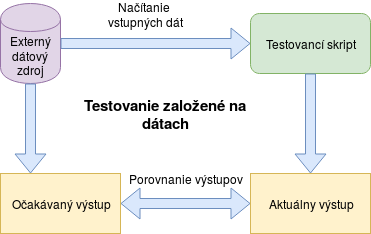
\includegraphics[width=3.5in,height=2.2in]{obrazky-figures/Data-driven_testing.png}\\[1pt]
	\caption{Diagram záladnej štruktúry testovania založeného na dátach .}
	\label{Tdd_img}
\end{figure*}
\section{Editácia a uloženie testovacích dát}
Využívané testovacie dáta sa všeobecne skladajú z kombinácie vstupných a očakávaných výstupných dát. Daný typ dát sa najlepšie popisuje formou {\it rozhodovacích tabuliek}. Rozhodovacia tabuľka v najjednoduchšej forme poskytuje vstupy ako aj očakávané výstupy na jednom riadku. Pri tvorbe tabuľky je dôležitá správna identifikácia všetkých vstupných dát a ich rozdelenie do {\it domén}. Výber konkrétnych hodnôt záleží od zvoleného prístupu \cite{Ast}. Najčastejšie sa využívajú nasledovné prístupy:
\begin{itemize}
	\item{ \textit{Testy pokrývajúce logiku}. Testovacie prípady spoločne dosahujú všetky definované výstupy a rovnako zaručujú vykonanie všetkých častí kódu minimálne raz.}
	\item{ \textit{Rozdelenie na ekvivalenčné triedy} \ref{ekv_tr}. 
		Vstupy sa rozdeľujú  do tried za účelom redukcie počtu testov. Predpokladá sa, že test s jedným prvkom triedy reprezentuje všetky ostatné. }
	\item{ \textit{Analýza hraničných hodnôt}. 
		Prístup využíva ekvivalenčné triedy, jednotlivých reprezentantov ale nevolí náhodne. Keďže najčastejšie chyby sa vyskytujú pri hraničných hodnotách, konkrétne hodnoty volí z hraničných oblastí. Zohľadňuje pritom vstupné aj výstupné dáta.}
	\item{ \textit{Grafy príčin a dôsledkov (angl. Cause-Effect Graph)} \ref{ceg}. 
		Vytvárajú logickú grafovú reprezentáciu medzi požiadavkami a výsledkami testov. Pomáhajú pri výbere účelných a úplných testov.}
\end{itemize}


Vzhľadom k charakteru dát sa k ich editácii prirodzene ponúka použitie tabuľkových procesorov (anglicky{\it spreadsheet}). Prácu s danými programami obvykle zvládajú testeri, ale aj ľudia z oblasti biznisu, čo uľahčuje ich rýchle zapojenie. Dané programy sa často používajú aj na jednoduchý manažment testov pre manuálne testovanie. V tomto prípade sa dáta môžu zdieľať s automatizovanými testami a predchádzať tak ich zbytočnej redundancii. Príklad tabuľky je uvedený na obrázku \ref{Domtab_img}. 
\begin{figure*}[h]\centering
	\centering
	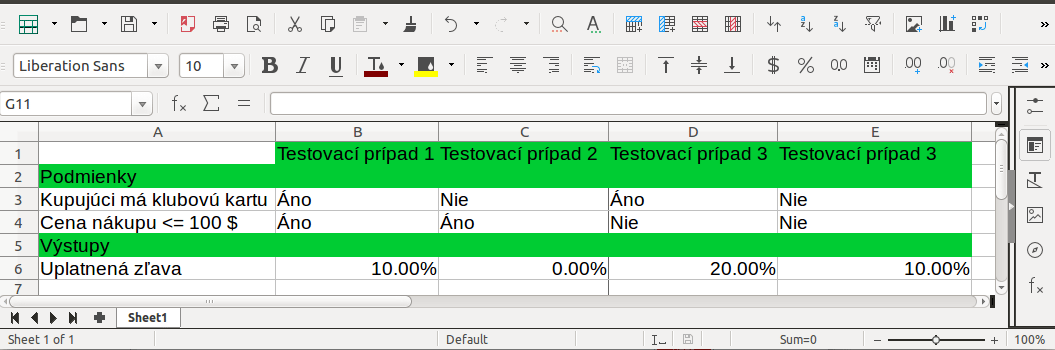
\includegraphics[width=6.0in,height=2.2in]{obrazky-figures/decision_table.png}\\[1pt]
	\caption{Príklad rozhodovacej tabuľky pre uplatnenie zľavy vytvorenej v tabuľkovom editore.}
	\label{Domtab_img}
\end{figure*}

Formáty uloženia tabuliek spadajú do viacerých kategórií. Jednoduchý databázový súbor (anglicky flat file database) je jednoduchá databáza (väčšinou tabuľka) uložená v textovom súbore ve forme krátkeho textu. Obvykle používané formáty sú napríklad hodnoty oddelené čiarkami (CSV), hodnoty oddelené tabulátormi (CSV, TXT) alebo iný špecifický formát (variácie XLS). Rovnako sú stále viac používané štrukturované formáty ako XML a Json. Súčasné programovacie jazyky majú knižnice pre ich načítanie a spracovanie, čo výrazne uľahčuje ich využitie. Jednoduché dabázové súbory môžu mať problémy pri výraznom rozširovaní. Rovnako je v nich neprehľadné uchovávanie rôznych konfigurácií a verzií. 

Pre veľké množstvo testovacích dát je vhodné použitie relačnej databázy. Umožňuje editáciu prostredníctvom skriptov ako aj pomocou grafických editorov.       


\section{Ekvivalenčné triedy a kritéria pokrytia}
\label{ekv_tr}
Zmyslom tvorby testovacích prípadov je nájdenie vstupov, ktoré najlepšie pokrývajú zvolené kritérium pokrytia. V závislosti od zložitosti testovaného softvéru môže byť množstvo možných vstupov  potenciálne nekonečné, preto je zvolenie vhodnej množiny testovacích dát náročné \cite{Gst}.
\subsection*{Rozdelenie vstupných domén na ekvivalenčné triedy}
Kľúčová je správna identifikácia vstupných domén. {\it Vstupná doména} testovaného systému je definovaná množinou všetkých vstupných hodnôt, ktoré nadobúda. V závislosti na testovacej úrovni a testovaného artefaktu sú to obvykle parametre metód, statické a globálne premenné, objekty reprezentujúce stav systému, užívateľské vstupy a argumenty programu \cite{Ist}. Vstupná doména je následne rozdelená na {\it ekvivalenčné triedy} (označované aj ako bloky). Pojem ekvivalencie sa definuje za predpokladu, že všetky hodnoty v jednej triede obsahujú z pohľadu testovania rovnako užitočné hodnoty. Každý prvok patrí práve do jednej triedy a jediný prvok z ekvivalenčnej množiny reprezentuje všetky prvky. Keď overíme testovací prípad pre jeden prvok, predpokladáme, že sme overili všetky prvky z danej množiny. 

Pri rozpade domény \(D\) podľa rozdelenia \(q\) vznikajú vzájomne disjunktné ekvivalenčné triedy (bloky) \(B_{q}\)  definované nasledovne:

\begin{center}
	\(b_{i} \cap b_{j} = \emptyset , i \neq j ; b_{i} , b_{j} \in B_{q}\)
\end{center}


a spolu pokrývajú doménu \(D\)

\begin{center}
	\( \underset{b \in B_{q}}  \bigcup b = D\)
\end{center}
%\begin{figure*}[h]\centering
%	\centering
%	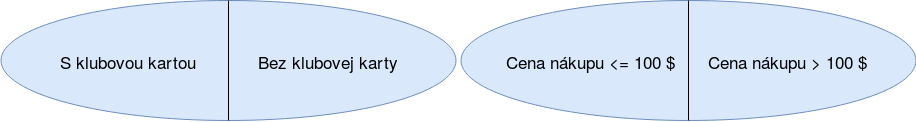
\includegraphics[width=6.5in,height=1.0in]{obrazky-figures/Domeny_dia.png}\\[1pt]
%	\caption{Rozpad domén z tabuľky \ref{Domtab_img} na ekvivalenčné triedy}
%	\label{Domdia_img}
%\end{figure*}
\begin{figure*}[h]\centering
	\centering
	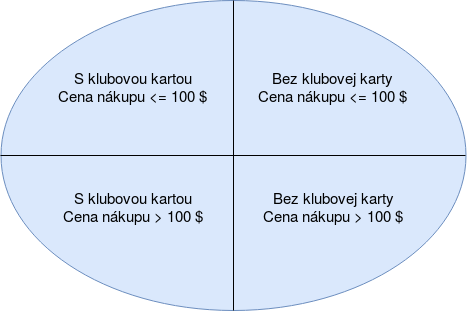
\includegraphics[width=3.5in,height=2.2in]{obrazky-figures/Domeny_all_dia.png}\\[1pt]
	\caption{Rozpad domén z tabuľky \ref{Domtab_img} na ekvivalenčné triedy}
	\label{Domdia_img}
\end{figure*}
\subsection*{Kritéria pokrytia}
Po identifikácií vstupných blokov je ďalším krokom vytvorenie konkrétnej testovacej sady. Efektívne testovanie množstva blokov vyžaduje vhodný výber ich kombinácií. Stratégie zvolenia kombinácií sú dané konkrétnym kritériom pokrytia. \textit{Kritérium pokrytia (angl. Coverage criterion)} je pravidlo alebo predpis pre systematické generovanie požiadavkov na test. \textit{Pokrytie (angl. coverage)} je miera udávajúca, ako veľmi daná testovacia sada skúma testovaný systém. Obvykle sa udáva v percentách a viaže sa na konkrétne kritérium \cite{Ist}.     
\begin{itemize}
	\item{ \textit{Kritérium pokrytia všetkých kombinácií(angl. All Combinations Coverage)}. Kritérium vyžaduje pokrytie všetkých kombinácií blokov zo všetkých domén. Testovacie prípady spoločne dosahujú všetky definované výstupy a rovnako zaručujú vykonanie všetkých častí kódu minimálne raz. Reálne sa dá použiť len pri minimálnom množstve blokov.
	}
	\item{ \textit{Kritérium pokrytia všetkých párov blokov (angl.  Pair-Wise Coverage)}. Kritérium vyžaduje kombináciu každého bloku každej domény s každým blokom každej inej domény, teda všetkých dvojíc blokov z rôznych domén. Generalizáciou kritéria je \textit{Kritérium pokrytia všetkých n-tíc blokov (angl. T-Wise Coverage).}  
	}
	\item{ \textit{Kritérium pokrytia bázových blokov (angl. Base Choice Coverage)}. Pre každú doménu je zvolený bázový blok,  zvyčajne ide o najčastejší alebo najdôležitejší blok. Kritérium vyžaduje kombinácie všetkých bázových blokov každej domény a pokrytie každého nebázového bloku. Vhodne zvolené kombinácie bázových blokov výrazne redukujú celkový počet testovacích prípadov. Vyšší stupeň predstavuje \textit{Kritérium pokrytia viacerých bázových blokov (angl. Multiple Base Choices Coverage)} 
	} 	
	\item{ \textit{Kritérium pokrytia každého bloku (angl. Each Choice Coverage)}. Kritérium vyžaduje pokrytie každého bloku pre každú doménu. Minimálny počet testov sa rovná počtu blokov. Kritérium nie je veľmi efektívne a samotnú voľbu testovacích prípadov necháva na testerovi. Nevyžaduje žiadnu kombináciu hodnôt a preto je považované za slabé.
	}
\end{itemize}


\section{Grafy príčin a dôsledkov}
\label{ceg}
Slabinou predstaveného prístupu založeného na rozklade na ekvivalenčné triedy je absencia kombinácií vstupov. Riešenie ponúkajú spomenuté kritéria pokrytia, ale počet kombinácií vstupných dát je napriek tomu obvykle príliš vysoký. \textit{Graf príčin a dôsledkov (angl. Cause-Effect Graphing, CEG)} je grafický spôsob znázornenia prepojenia vstupov \textit{(príčiny, angl. causes)} s nimi asociovanými výstupmi \textit{(dôsledky, angl. effects)}. Graf je formálne vyjadrenie boolovských požiadaviek a umožňuje systematický spôsob výberu podmnožiny testovacích prípadov. 
Výhody prístupu sú nasledovné:
\begin{itemize}
	\item{ Redukcia počtu kombinácií vstupov
	}
	\item{ Odhalenie nejasností a nekompletnosti špecifikácie
	}
	\item{ Zrozumiteľný a jasne čitateľný formát
	}
	\item{ Zlepšenie celkového chápania systému a jeho dôležitých faktorov 
	} 	
	\item{ Pomoc pri hľadaní zdroja konkrétnej príčiny a dôsledkov  
	} 	
\end{itemize}
Pre tvorbu testovacích prípadov je použitý nasledovný proces \cite{Ast}:
\begin{enumerate}
	\item{ \textit{Rozdelenie požiadavkov do skupín primeranej veľkosti.} Veľké množstvo požiadaviek by vyústilo do príliš veľký grafu, ktorý sa stane nepoužiteľným. 
	}
	\item{ \textit{Identifikácia príčin a dôsledkov.} Príčina je priamo vstupná podmienka alebo jej ekvivalenčná trieda. Dôsledok je výstupná podmienka alebo zmena v systéme.  
	} 	
	\item{ \textit{Analýza významu požiadavkov a vytvorenie grafu príčin a dôsledkov.} 
	} 
	\item{ \textit{Identifikácia obmedzení medzi príčinami a dôsledkami.} 
	} 
	\item{ \textit{Konvertovanie grafu do rozhodovacej tabuľky.} 
	}  	
	\item{ \textit{Každý stĺpec v tabuľke reprezentuje testovací prípad.}
	}  		
\end{enumerate}

\subsection*{Notácia grafu}
Základná notácia grafu je ukázaná na obrázku \ref{ceg_img}. Každý uzol môže nadobúdať hodnoty 0 a 1 reprezentujúce absenciu a prítomnosť stavu. Celkovo syntax pokrýva štyri prípady \cite{Ast}: 
\begin{itemize}
	\item{Funkcia \textit{identity}: ak \(a = 1\) tak \(b = 1\), inak \(b = 0\) 
	}
	\item{Funkcia \textit{NOT}: ak \(a = 1\) tak \(b = 0\), inak \(b = 1\) 
	}
	\item{Funkcia \textit{OR}: ak \(a\), \(b\) alebo \(c\) je rovné \(1\), tak \(d = 1\) 
	} 		
	\item{Funkcia \textit{AND}: ak \(a = 1\) a súčastne \(b = 1\), tak \(c = 1\), inak \(c = 0\)  
	} 
\end{itemize}
\begin{figure*}[h]\centering
	\centering
	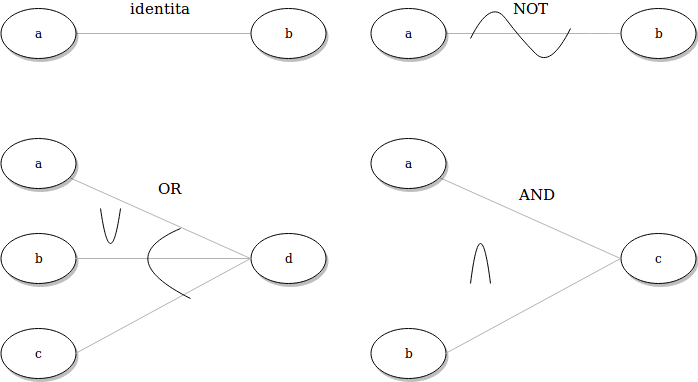
\includegraphics[width=4.5in,height=2.2in]{obrazky-figures/ceg.png}\\[1pt]
	\caption{Základné symboli CEG grafu \cite{Ast}.}
	\label{ceg_img}
\end{figure*}
Niektoré kombinácie medzi príčinami a dôsledkami sú neuskutočniteľné. Grafová reprezentácia na obrázku \ref{ceg_cons_img} preto umožňuje obmedzenia popísať nasledovne \cite{Ast}:
\begin{itemize}
	\item{Obmedzenie \textit{E}: Najviac jeden z uzlov \(a\) a \(b\) je súčasne rovný \(1\) 
	}
	\item{Obmedzenie \textit{I}: Aspoň jeden z uzlov \(a\), \(b\) a \(c\) je vždy rovný \(1\) 
	}
	\item{Obmedzenie \textit{O}: Práve jeden z uzlov \(a\) a \(b\) je  rovný \(1\) 
	} 		
	\item{Obmedzenie \textit{R}: Aby \(a\) mohlo byť \(1\), \(b\) musí byť \(1\) 
	}
\end{itemize}    
\begin{figure*}[h]\centering
	\centering
	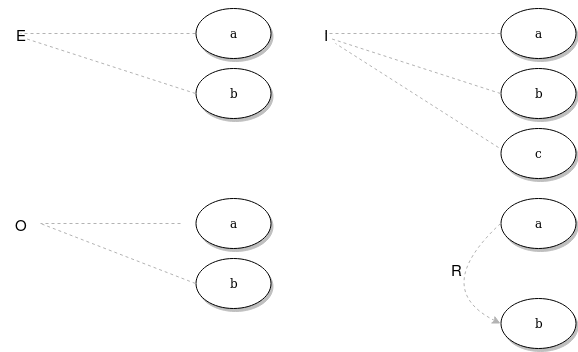
\includegraphics[width=4.5in,height=2.2in]{obrazky-figures/ceg_cons.png}\\[1pt]
	\caption{Základné symboli CEG grafu \cite{Ast}.}
	\label{ceg_cons_img}
\end{figure*}

\section{Testos}
\label{Testos}
Platforma \textit{Testos} (Test Tool Set) \cite{Testos} je projekt, ktorého hlavným cieľom je vytvorenie ucelenej sady nástrojov podporujúcich automatizované testovanie softvéru. Platforma sa sústreďuje na všetky úrovne testovania a podľa zamerania je rozdelená na oblasti:
\begin{itemize}
	\item{Testovanie grafického užívateľského rozhrania \textit{(GUI)}
	}
	\item{Testovanie založené na modeloch \textit{(Model-based)}
	}
	\item{Testovanie založené na požiadavkách \textit{(Requirement-based)}
	} 	
	\item{Testovanie založené na dátach \textit{(Data-based)}
	} 	
	\item{Dynamická analýza \textit{(Execution-based)}
	} 	
\end{itemize}  
Oblasť testovania založeného na dátach aktuálne obsahuje nástroje pre generovanie testovacích dát pre databázy (náhodné dáta, kombinácie dát a ich mutácie), detektory databázovej štruktúry a detektory štrukturovaných dát. Nástroj vytvorený v diplomovej práci patrí do rovnakej oblasti, v rámci nej priamo komunikuje a využíva ostatné nástroje Testos.

\begin{figure*}[h]\centering
	\centering
	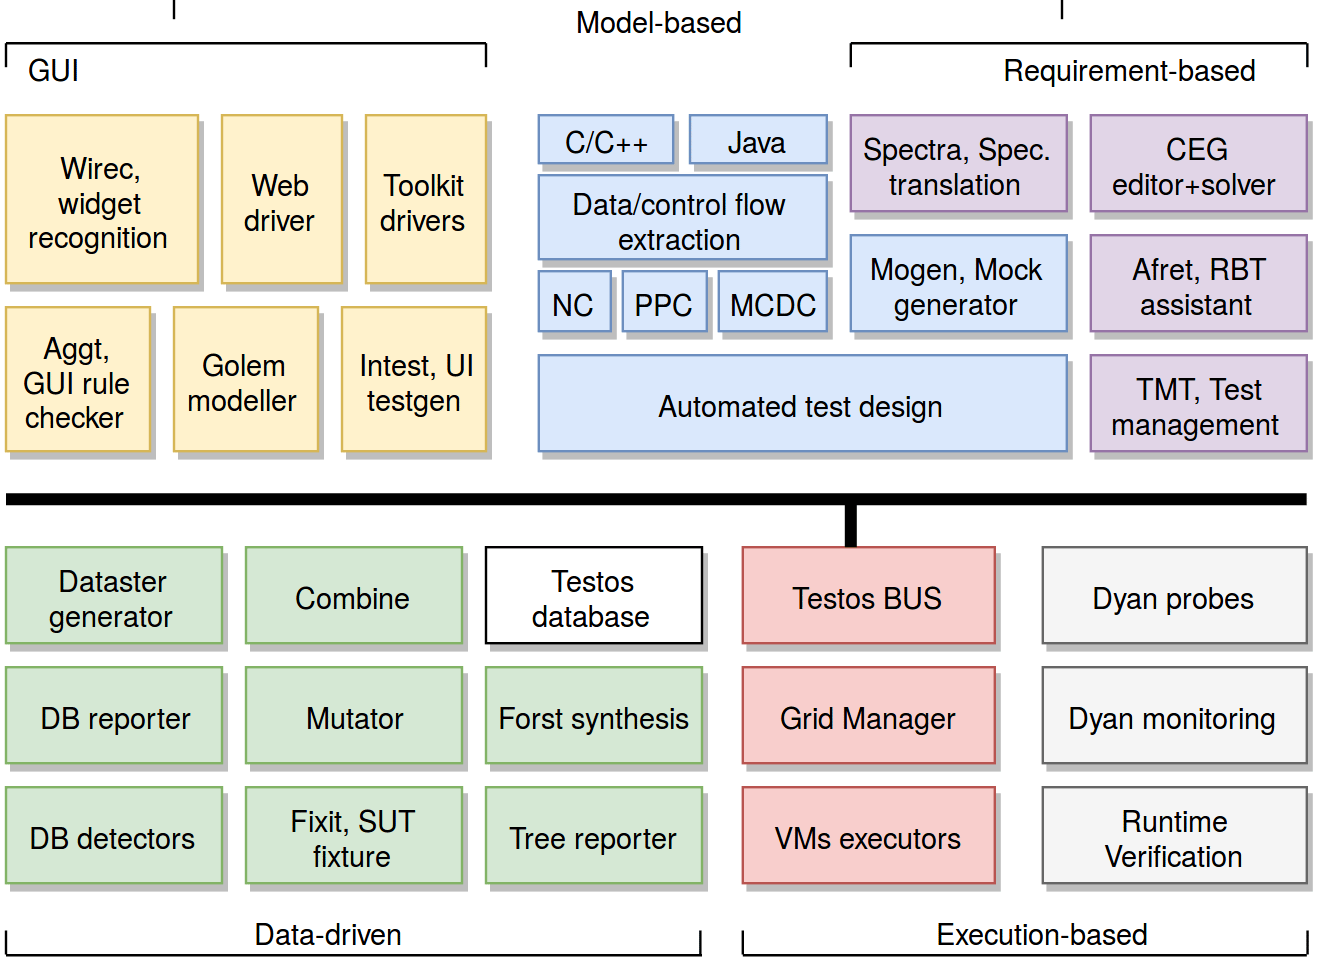
\includegraphics[width=6.0in,height=4.2in]{obrazky-figures/testos.png}\\[1pt]
	\caption{Platforma Testos \cite{Testos}.}
	\label{testos_img}
\end{figure*} 


\chapter{Štrukturované dáta} 
\label{struktury}

Disponovanie vhodnými \textit{testovacími dátami} je pre proces testovania rovnako dôležité ako konkrétne prípady. S narastajúcou veľkosťou a komplexnosťou systémov je získanie takýchto dát stále obtiažnejšie. V danej kapitole je najskôr uvedená všeobecná charakteristika štrukturovaných dát a spôsob ich grafovej reprezentácie. Ďalej sa rozoberá problematika  porovnania stromových dát z pohľadu štruktúry. Nakoniec poskytne prehľad používaných formátov a existujúcich riešení získania testovacích dát.


\section{Stromové štruktúry}
V informatike je \textit{stom} je nelineárna dátová štruktúra, ktorá predstavuje stromovú štruktúru s prepojenými uzlami. Prvky v strome sú hierarchicky usporiadané, poskytujú prirodzenú organizáciu dát a sú všadeprítomné v súborových systémoch, databázach, grafických užívateľských rozhraniach, webových stránkach a iných počítačových systémoch. 

Stromová dátová štruktúra \(T\) je rekurzívne definovaná ako množina \textit{uzlov}, kde každý uzol je dátová štruktúra. Uzly sú vo vzťahu \textit{rodiča s potomkom (angl. parent-child)}, ktorý je definovaný nasledovne \cite{Dsaj}:
\begin{itemize}
	\item{Ak je \(T\) neprázdna, tak obsahuje práve jeden špeciálny uzol označovaný ako \textit{koreňový (angl. root)} ktorý nemá žiadny rodičovský uzol.
	}
	\item{Každý uzol \(v\) množiny \(T\) má priradený \textit{rodičovský} uzol \(w\). Každý uzol s rodičom \(w\) je jeho potomkom.
	}	
\end{itemize}
Ďalšie prvky v strome:
\begin{itemize}
	\item{Dva uzly sú \textit{súrodenci (angl. siblings)}, pokiaľ majú rovnakého rodiča.
	}
	\item{Uzol je \textit{koncový}, ak nemá žiadnych potomkov. Externé uzly sú tiež označované ako \textit{listy(angl. leafs)}. 
	}
	\item{Uzol, ktorý má aspoň jedného potomka je \textit{vnútorný (angl. internal)}.
	}	
	\item{\textit{Podstrom (angl. subtree)} stromu \(T\) je strom \(S\) tvorený uzlom z \(T\) a všetkými jeho potomkami
	}		
\end{itemize} 
\subsection*{Porovnanie stromov}
Analýza dát je proces inšpekcie, očistenia a transformácie dát s cieľom získania užitočných informácií. S analýzou stromových dát súvisia problémy inklúzie stromov, vzdialenosť stromov, hľadanie spoločných podstromov a iné. Pre potreby nástroja vytvoreného v rámci tejto práci sú pre ich zložitosti nevhodné.

Základná operácia nad každou množinou je prienik. Pri stromoch jeho hľadanie začína od koreňového uzla. Obrázok \ref{intersection_img} znázorňuje prienik troch stromov. Pre účely nástroja je zistenie prieniku schémy stromov užitočná operácia. Vstupná doména, reprezentovaná stromovou štruktúrou, umožňuje v prípade detekcie zhodných častí rôznych stromov tieto časti agregovať. Tým zmenšuje množinu príčin CEG \ref{ceg}. Obrázok \ref{intersection_img} znázorňuje redukciu množiny príčin odstránením irelevantných prvkov.
\begin{figure*}[h]\centering
	\centering
	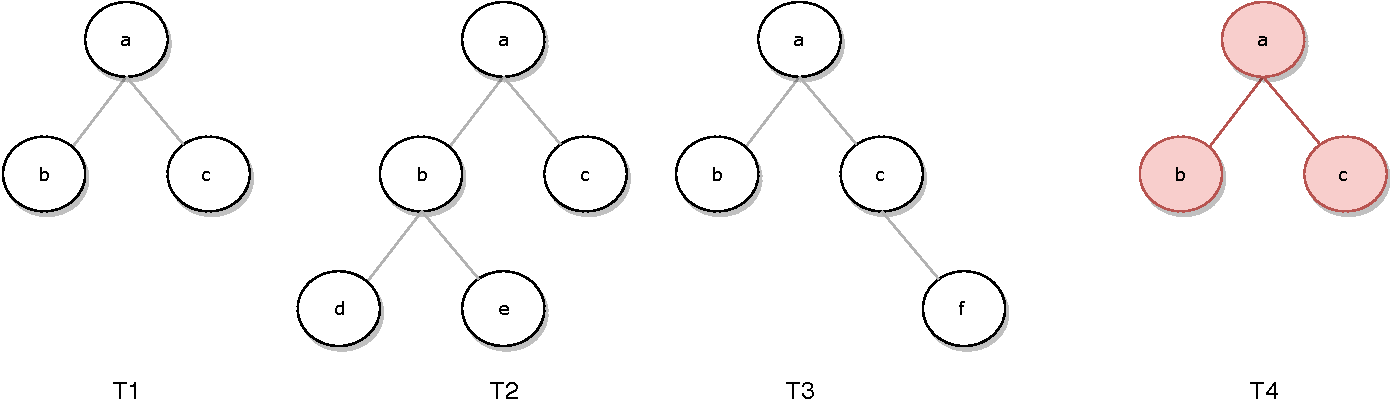
\includegraphics[width=6.0in,height=2.0in]{obrazky-figures/tree_intersection.pdf}\\[1pt]
	\caption{Prienik troch stromov.}
	\label{intersection_img}
\end{figure*} 
\begin{figure*}[h]\centering
	\centering
	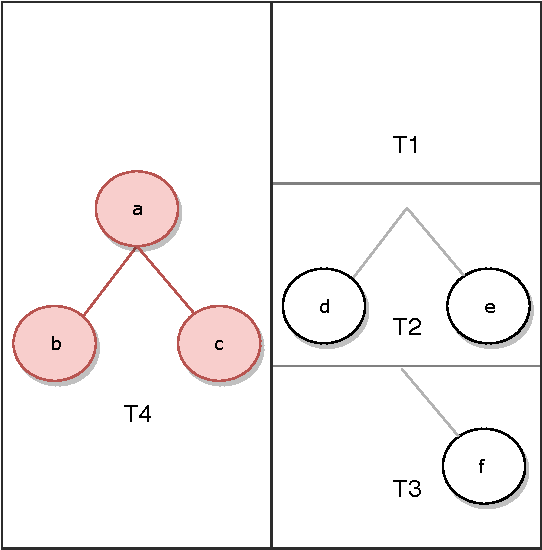
\includegraphics[width=2.8in,height=3.0in]{obrazky-figures/cause_intersection.pdf}\\[1pt]
	\caption{Redukcia množiny príčin CEG.}
	\label{intersection_img}
\end{figure*} 

Porovnávanie stromov sa dá rozdeliť do troch kategórií na základe stromovej \textit{štruktúry, sémantiky} hodnôt uzlov a oboch zároveň. Zistenie sémantiky hodnôt v uzloch nieje predmetom tohto nástroja, ale inej komponenty vrámci platformy Testos.  
\section{Prehľad serializačných formátov}
Serializácia dát je proces konverzie štrukturovaných dát a objektov do formátu, ktorý umožňuje ich uloženie alebo zdieľanie. Deserializácia je k nej opačný proces, pri ktorom sa zo štrukturovaných dát v určitom formáte rekonštruujú dáta do pôvodnej formy. V niektorých prípadoch sa serializácia používa aj so zámerom zmenšenia množstva dát, ktoré sa ukladá alebo prenáša. V tejto sekcii sú predstavené dva najpoužívanejšie serializačné formáty.        
\subsection*{XML}
\textit{XML (Extensible Markup Language)} je \textit{značkovací jazyk} dokumentov ako aj formát výmeny dát, ktorý vychádza z princípov jazyka SGML. Značkovací jazyk je systém pre značenie častí dokumentov, ktoré indikujú jeho logickú štruktúru. XML tiež umožňuje definovať časti informácií v štrukturovanom formáte.XMLdef

XML dáta sami uchovávajú ich popis a definíciu. Štruktúra je obsiahnutá v dátach, preto nieje potrebné ju najskôr vytvoriť a následne naplniť. Základný stavebný blok XML dokumentu je \textit{prvok(angl. element)}, definovaný \textit{značkami(angl. tag)}. Každý element má začínajúci a ukončujúci tag. Ku značkám môžu byť uložené metadáta vo forme \textit{atribútov(angl. attributes)}. Elementy môžu byť vnorené, čo umožňuje reprezentáciu hierarchickej štruktúry. Názov elementu popisuje jeho obsah a štruktúra jeho vzťahy k ostatným. Všetky elementy sa nachádzajú vo vonkajšom elemente, nazývanom \textit{koreňový(angl. root)}\cite{XMLdef}.      
\subsection*{JSON}
\textit{JSON (JavaScript Object Notation)} je formát pre výmenu dát, ktorý vychádza z podmnožiny programovacieho jazyka \textit{Javascript}. Formát JSON je odľahčený, ľahko čitateľný a zapisovateľný človekom a nezávislý na konkrétnom programovacom jazyku.

JSON sa skladá z dvoch typov štruktúr, ktoré sú podporované vo väčšine súčasných programovacích jazykoch. Kolekcia dvojíc kľúč/hodnota sa nazýva \textit{objekt(object)} a je reprezentovaná v rôznych jazykoch dátovými typmi objekt, slovník, hašovacia tabuľka či asociatívne pole. Objekt začína a končí zloženými zátvorkami \textit{\{\}}, kľúč má dátový typ \textit{reťazec(string)}. Druhá štruktúra je zoradený zoznam hodnôt \textit{pole(array)}. Pole je ohraničené hranatými zátvorkami \textit{[]}, jednotlivé hodnoty sú oddelené čiarkou. Dátové typy hodnôt sú \textit{string, number, object, array, true, false, null}\cite{JSONdef}.  

\subsection*{Porovnanie XML a JSON}
XML vytvorené v roku 1998 bolo dlho jedinou voľbou pre serializáciu a prenos dát. JSON bol špecifikovaný v roku 2001 a spočiatku sa ťažko presadzoval. Postupne sa dominancia XML znižuje a JSON sa stáva preferovanejší formát pre webové rozhrania \ref{xml_vs_json_img}. Hlavné rozdiely formátov sú uvedené v nasledujúcich bodoch.
\begin{itemize}
	\item{\textbf{Kompaktnosť}: JSON pri popise dát využíva menej znakov a preto je výsledný súbor pri serializácii rovnakých dát menší.
	}	
	\item{\textbf{Čitateľnosť}: Oba formáty sú dobre čitateľné človekom. JSON je jednoduchší a obsahuje menej zbytočných dát, preto je ľahšie čitateľný.
	}
	\item{\textbf{Rýchlosť spracovania}: Softvér na spracovanie XML dát je pomalší a ťažkopádny. Knižnice pracujúce s DOM pre zložitosť XML spracovania a jeho mnohovravnosti často využívajú nadmerné množstvo pamäte.
	}
	\item{\textbf{Štruktúra}: JSON dáta majú štruktúru mapy a XML dáta stromu. JSON dáta môžu byť prevedené na XML, opačne to bez straty informácii nieje možné.
	}	
	\item{\textbf{Typické dáta}: JSON je lepší pre prenos dát. XML je lepší pre prenos dokumentov, kde poskytuje rôzne pohľady na rovnaké dáta.
	}	
\end{itemize}   
\begin{figure*}[h]\centering
	\centering
	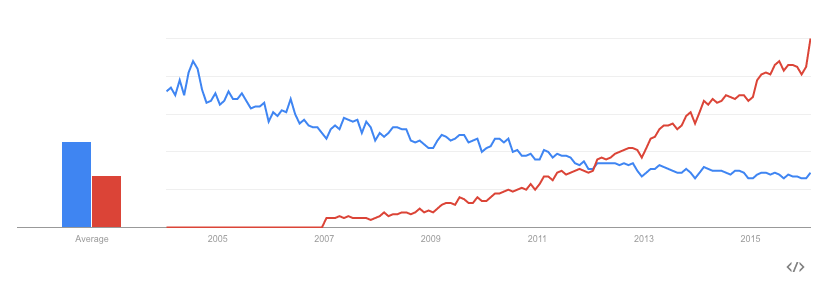
\includegraphics[width=\textwidth,height=\textheight,keepaspectratio]{obrazky-figures/xml_vs_json.png}\\[1pt]
	\caption{Graf znázorňujúci trendy vyhľadávania google pre výrazy  ‘json api’ (červené) a ‘xml api’ (modré).\cite{XMLvsJSONusage}}
	\label{xml_vs_json_img}
\end{figure*} 
\section{Existujúce riešenia}
Práca nadväzuje na nástroj \textit{StructAnalyser}, ktorý vznikol v rámci bakalárskej práce. Nástroj je unikátny z pohľadu analýzy vzoriek dát bez znalosti ich štruktúry pre testovacie účely. Iné nástroje sú odlišné v účeloch a znalostiach, preto stanoveným požiadavkám nevyhovujú. 

Existujúce nástroje vykonávajúce analýzu vzoriek dát sa dajú rozdeliť do kategórií podľa účelu analýzy a znalosti štruktúry dát. Najviac zastúpené nástroje sú zamerané na zisk biznis informácií so znalosťou ich štruktúry. Typicky pracujú s dátovými skladmi. Druhú početnú skupinu predstavujú nástroje pre účely testovania so znalosťou štruktúry dát a zdrojového kódu programu. Platforma Testos má nástroje pre analýzu databázy a následné generovanie testovacích dát. Nutná podmienka ich použitia je znalosť štruktúry databázy.
\subsection*{Nástroj StructAnalyser}
Nástroj \textit{StructAnalyser} analyzuje štrukturované dáta v často používaných formátoch JSON a XML. Slúži k agregácií vstupných dát, určeniu váhy jednotlivých dátových entít a abstrakcii skalárnych hodnôt. Rovnako podporuje generáciu dát podobných vstupným vzorkám.
Nástroj je implementovaný ako konzolová aplikácia. Pri spustení vyžaduje nasledovné argumenty\cite{BPgen}.
\begin{itemize}
	\item{\textit{-input}: Súbor so vstupnými dátami. Dáta sú v jednom z formátov XML, JSON alebo YAML.
	}	
	\item{\textit{-c}: Konfiguračný súbor vo formáte JSON. Obsahuje špecifikáciu abstrakcie hodnôt a uzlov. Parameter je voliteľný.
	}	
	\item{\textit{-g}: Prepínač udávajúci výstup vo forme generovaných hodnôt. Prijíma čislo určujúce počet vygenerovaných entít.
	}	
\end{itemize} 
\begin{figure*}[h]\centering
	\centering
	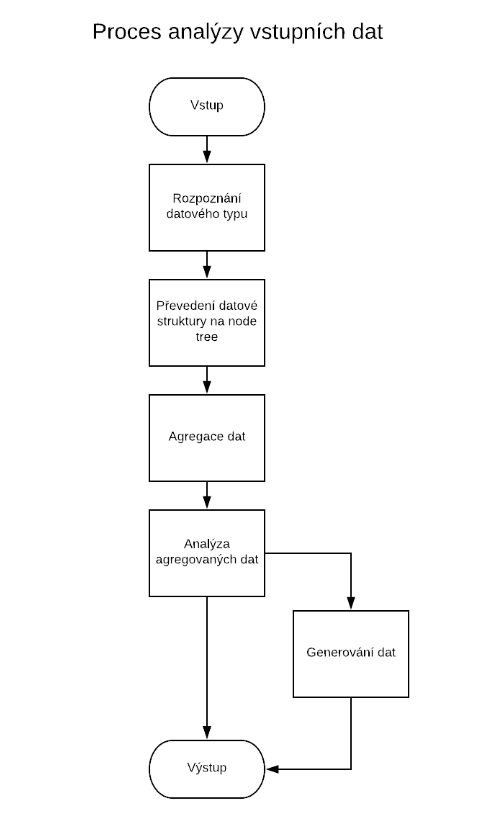
\includegraphics[width=3.0in,keepaspectratio]{obrazky-figures/struct_analyser.png}\\[1pt]
	\caption{Proces spracovania vstupných dát na výstupnú analýzu nástroja \textit{StructAnalyser}\cite{BPgen}}
	\label{structa_img}
\end{figure*} 
Nástroj funguje samostatne a poskytuje očakávanú funkcionalitu, ale má aj slabé stránky.
\begin{enumerate}
	\item{Chýbajúca \textit{spolupráca s nástrojmi v rámci platformy Testos.} Detektory implementované v nástroji sú obmedzené a ťažko rozšíritelne. Rovnako obmedzený je aj generátor dátových entít. V platforme Testos sú nástroje na generáciu a detekciu .   
	}
	\item{\textit{Štatistická abstrakcia konkrétnych štruktúr.} Nástroj neuchováva vzory štruktúr spracovaných dát. Generátor následne vytvára vzorky dát len na základe štatistiky, čím dochádza k generovaniu nezmyselných štruktúr.
	} 	
	\item{\textit{Abstrakcia hodnôt koncových uzlov.} Obmedzené detektory dôkladne neskúmajú hodnoty. Rovnako sa stráca informácia o hodnotách uzlov konkrétnych štruktúr.
	} 
		
\end{enumerate}



\chapter{Návrh nástroja pre detekciu závislostí stromových štruktúr}
\label{navrh}
V prvej časti tejto kapitoly sú spracované požiadavky na vytváraný nástroj pre detekciu závislostí stromových štruktúr pre účely testovania. Druhá časť obsahuje návrh architektúry a postup detekcie závislostí. Vytváraný nástroj je ďalej tiež referovaný pod názvom \textit{TSD analyser}.
\begin{figure*}[h]\centering
	\centering
	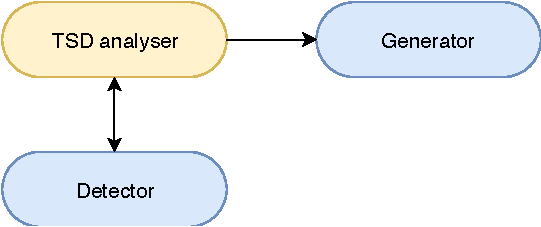
\includegraphics[width=3.0in,keepaspectratio]{obrazky-figures/testos_components.pdf}\\[1pt]
	\caption{Diagram nástrojov platformy Testos, ktoré budú využité pri procese analýzy a generovania testovacích stromových dát.}
	\label{testos_nastroje}
\end{figure*} 
\section{Špecifikácia požiadaviek}
Táto podkapitola obsahuje požiadavky na výsledný nástroj \textit{TSD analyser}. V tabuľke \ref{rq_general} najskôr uvádza základné požiadavky, ktoré sú ďalej podrobnejšie špecifikované. 

%\section{Špecifikácia požiadavkov}
\begin{table}[hbt]
	\centering
	\label{rq_general}
	\begin{tabular}{|p{0.8cm}|p{15cm}|}
		\hline
		\textbf{Číslo} & \textbf{Popis požiadaviek} \\ \hline
		1 & Nástroj spolupracuje s ďalšími nástrojmi Testos \\ \hline
		2 & Nástroj vytvára abstrakciu štruktúr vzoriek dát \\ \hline
		3 & Nástroj získa abstrakciu sémantiky hodnôt uzlov \\ \hline
		4 & Nástroj umožňuje simultánne skúmať dvojíc vzoriek stromových štruktúr \\ \hline
		5 & Nástroj vytvára predpis pre generovanie dát \\ \hline
		6 & Nástroj overí zhodu vzorky dát s vopred vytvorenou abstrakciou \\ \hline
		7 & Nástroj poskytuje grafické rozhranie pre vizualizáciu abstrakcie  \\ \hline
	\end{tabular}
	\caption{Tabuľka základných požiadaviek}
\end{table}

\subsection*{Nástroj spolupracuje s ďalšími nástrojmi Testos}
Implementovaný nástroj implicitne komunikuje s ďalšími nástrojmi prostredníctvom REST API. Vzhľadom k komunikácii v rámci uzatvorenej platformy nieje vyžadovaná autentifikácia. Nástroj sám iniciuje spojenia a zadáva požiadavky ostatným nástrojom.   
\subsection*{Nástroj vytvára abstrakciu štruktúr vzoriek dát}
Abstrakcia štruktúry stromových dát tvorí jadro nástroja. Požiadavky na abstrakciu štruktúr sú v tabuľke \ref{rq_2}.  
\begin{table}[hbt]
	\centering
	\label{rq_2}
	\begin{tabular}{|p{0.8cm}|p{15cm}|}
		\hline
		\textbf{Číslo} & \textbf{Popis požiadaviek} \\ \hline
		2.1 & Nástroj obsahuje univerzálnu stromovú štruktúru \\ \hline
		2.2 & Nástroj uchováva všetky vzory štruktúr vzoriek dát \\ \hline
		2.3 & Nástroj zaznamenáva štatistiku výskytu unikátnych vzorov štruktúr \\ \hline	
		2.4 & Nástroj identifikuje spoločné časti štruktúr  \\ \hline
		2.5 & Nástroj agreguje polia koncových uzlov  \\ \hline	
		2.6 & Nástroj umožňuje uložiť a znovu obnoviť stav štruktúry  \\ \hline	
	\end{tabular}
	\caption{Tabuľka detailných požiadaviek abstrakcie štruktúr}
\end{table}
\subsection*{Nástroj získa abstrakciu sémantiky hodnôt uzlov}
Nástroj na abstrakciu sémantiky množiny hodnôt uzlov využíva komponentu platformy Testos. Detektor poskytuje sémantické informácie spolu s mieru príslušnosti.  Konkrétny význam týchto informácií nástroj nepozná.
\subsection*{Nástroj umožňuje simultánne skúmať dvojíc vzoriek stromových štruktúr}
Nástroj umožňuje súčasnú analýzu dvoch skupín vzoriek dát. Takéto dáta typicky predstavujú dvojicu vstupných a výstupných dát. Nástroj uchováva dvojice vzorov štruktúr, ktoré k sebe patria. 
\subsection*{Nástroj vytvára predpis pre generovanie dát}
Nástroj na syntézu testovacích dát využíva Testos komponentu Generator, pre ktorý vytvorí predpis štruktúry a sémantiky.
\subsection*{Nástroj overí zhodu vzorky dát s vopred vytvorenou abstrakciou}
Nástroj overí zhodu štruktúru vzorky s uloženými vzormi štruktúr. Rovnako overí jej sémantickú zhodu. 
\subsection*{Nástroj poskytuje grafické rozhranie pre vizualizáciu abstrakcie}
Grafické rozhranie poskytuje interaktívnu voľbu zobrazenia úrovne abstrakcie. Rovnako umožňuje editáciu sémantiky uzlov a výber konkrétnych vzorov pre generátor.  
\section{Architektúra}
%\section{Abstraktná stromová štruktúra}
V tejto podkapitole je rozobraný popis činností vyvíjaného nástroja \textit{TSD analyser}. Sú tu predstavené základné komponenty a ich kroky behu programu. 
\begin{figure*}[h]\centering
	\centering
	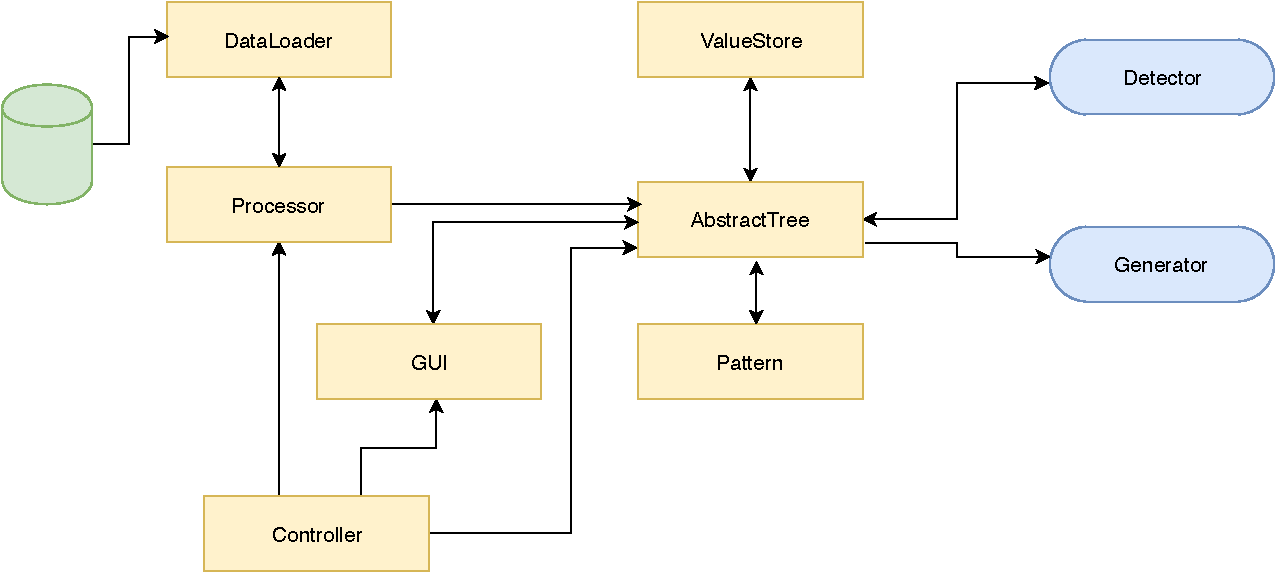
\includegraphics[width=6.0in,keepaspectratio]{obrazky-figures/architecture.pdf}\\[1pt]
	\caption{Diagram komponent nástroja TSD analyser spolu s nástrojmi Detector a Generator.}
	\label{architecture_img}
\end{figure*} 
\subsection*{DataLoader}
Komponenta DataLoader vykonáva načítanie vstupných vzoriek dát. Na vstupe má súbor so serializovanými dátami vo formáte XML alebo JSON. V prípade, že sú vo formáte XML, je tento formát konvertovaný na JSON. Samotné načítanie sa vykoná po žiadosti komponenty \textit{Preprocessor} o ďalšie dáta. 
\subsection*{Processor}
Processor je zodpovedný za prenos dát od DataLoader do ďalšej komponenty AbstractTree. Podľa nastavenia buď aktualizuje abstraktný strom, alebo overí zhodu vzorky dát s vopred vytvorenou abstrakciou. 
\subsection*{AbstractTree}
Jadrom celého nástroja je komponenta AbstractTree, uchovávajúca univerzálnu stromovú štruktúru \textit{Abstraktný dátový strom}. Je vytvorená zo všetkých štruktúr vzoriek a skladá sa z uzlov AbstractNode.   
\subsection*{ValueStore}
ValueStore uchováva všetky hodnoty uzlov vzoriek. Uložené dáta sa skladajú zo štvorice \textit{ID vzorky, ID uzla, dátového typu a hodnoty.}  
\subsection*{Pattern}
Komponenta Pattern skladuje všetky unikátne vzory štruktúr. Popis týchto vzorov sa odkazuje na abstraktný strom.
\subsection*{Controller}
Controller načítava konfiguračný súbor a je zodpovedný za jej distribúciu do ostatných komponent. Tiež riadi a synchronizuje činnosti ostatný komponent.
\subsection*{GUI}
GUI zabezpečuje grafickú vizualizáciu abstraktného stromu.  
\section{Abstraktný dátový strom} 
Algoritmus abstrakcie štruktúry vzoriek dát je založený na \textit{abstraktnom dátovom strome(ďalej označovaný AT).} Všetky vstupné vzorky sú prevedené do jedného hlavného AT. Tento strom sa skladá z \textit{abstraktných uzlov(ďalej označované AN)}. Táto kapitola obsahuje charakteristiku AT, AN a hlavné algoritmy, ktoré s nimi pracujú. 
\subsection*{Abstraktný uzol}
Abstraktné uzly \textit{AN} obsahujú tri typy informácií. Jednotlivé typy vychádzajú zo štruktúry jazyka JSON.   
\begin{enumerate}
	\item{\textbf{Object}: Uzol obsahuje nezoradenú množinu AN uzlov. 
	}	
	\item{\textbf{Value}: Uzol obsahuje konkrétnu hodnotu. 
	}	
	\item{\textbf{Array}: Uzol obsahuje množinu referencií na AT. 
	}		
	
\end{enumerate}
\subsection*{Algoritmus abstrakcie} 
Komponenty majú nasledovné množiny, ktoré algoritmus využíva pri abstrakcii.
\begin{itemize}
	\item{AbstractTree: \textit{Množina unikátnych vzorov}. Vzor je tvorený množinou uzlov \textit{AN} a ich typov.
	}
	\item{DataStore: \textit{Množina konkrétnych hodnôt AN typu Value}. Každý uzol z týchto uzlov si uchováva všetky konkrétne hodnoty, ktoré vo vzorkách dát nadobudol.
	}			
	\item{Pattern: \textit{Množina vzorov AT}. Konkrétny vzor dát sa skladá z množiny vzorov AT, ktoré ho tvoria.
	}					
\end{itemize}
Základné kroky algoritmu:
\begin{enumerate}

	\item{ Pomocou prehľadávania stromu do hĺbky \textit{(DFS)} získaj množinu uzlov \textit{AN} aktuálneho stromu \textit{AT}. Pri uzloch typu \textit{Array} ďalej nepokračuj v ich prehľadávaní a zaznamenaj ich.
	}
	\subitem{ Pokiaľ sa narazí na nový uzol, ktorý \textit{AT} ešte neobsahuje, vytvor ho. 
	}
	\subitem{ Pokiaľ je \textit{AN} typu \textit{Value}, ulož jeho konkrétnu hodnotu.
	}	
	\item{ Množina získaných uzlov vytvára konkrétny vzor daného \textit{AT}. Porovnaj tento vzor so všetkými doposiaľ získanými. Ulož identifikáciu získaného vzoru do množiny vzorov konkrétnej vzorky dát.
	} 
	\subitem{ Pokiaľ sa získaný vzor ešte nevyskytol, ulož ho medzi vzory daného stromu.
	}			
	\item{ Vyber prvý uzol z množiny \textit{Array}. Pokiaľ pre daný uzol ešte nebol vytvorený \textit{AT}, vytvor ho.   
	} 
	\item{ Pre každú hodnotu z vybraného \textit{Array} uzlu opakuj kroky 1 a 2. Ulož si identifikátory vzorov pre všetky hodnoty z uzla. } 
	}
	\item{ S množinou \textit{Array} uzlov nového stromu opakuj krok 3.} 
}  	  	
	\item{ Všetky uzly \textit{Array} boli spracované. Výsledné vzory všetkých \textit{AT} stromov zoraď ulož do komponenty Pattern.}
	}  	
	\item{ Hodnoty uzlov v komponente \textit{StoreData} odošli do nástroja \textit{Detector}. Ulož získané sémantické informácie.
	}
}  		
\end{enumerate}
\subsection*{Príklad práce algoritmu} 
Príklad práce algoritmu nad tromi vzorkami dát.\\
Vzorka dát č. 1:
\begin{lstlisting}
{"A":{"B":"ValueB","C":["ValueD",{"E":{"F":"ValueF"}}]}}
\end{lstlisting}
Vzorka dát č. 2:
\begin{lstlisting}
{"A":{"B":"ValueB2","G":"ValueG"}}
\end{lstlisting}
Vzorka dát č. 3:
\begin{lstlisting}
{"A":{"B":"ValueB","C":["VD","VD"]}}
\end{lstlisting}
Stav \textit{AT} po spracovaní prvej vzorky dát zobrazuje diagram \ref{alg_example1_img}. Číslo za identifikátorom \textit{AN} udáva jeho typ. Stav množín je v tabuľke \ref{alg_example1_tab}.
\begin{table}[hbt]
	\centering
	\label{alg_example1_tab}
	\begin{tabular}{|p{1.8cm}|p{12cm}|}
		\hline
		\textbf{Množina} & \textbf{Prvky} \\ \hline
		AT1 vzory & 	\(ATP1 = \{R1.1, A.1, B.2, C.3\}\) \\ \hline
		AT2 vzory & 	\(ATP2 = \{R2.2\}, ATP3 = \{R2.1, E.1, F.2 \}  \)   \\ \hline		
		Pattern & 	\(CP1 = \{ATP1, ATP2, ATP3\}  \)   \\ \hline
		DataStore & 	\(B.2 = \{"ValueB"\}, R2.2 = \{"ValueD"\}, F.2 = \{"ValueF"\}  \)   \\ \hline						

	\end{tabular}
	\caption{Tabuľka zobrazujúca stav množín po spracovaní prvého vzorku dát}
\end{table} 
\begin{figure*}[h]\centering
	\centering
	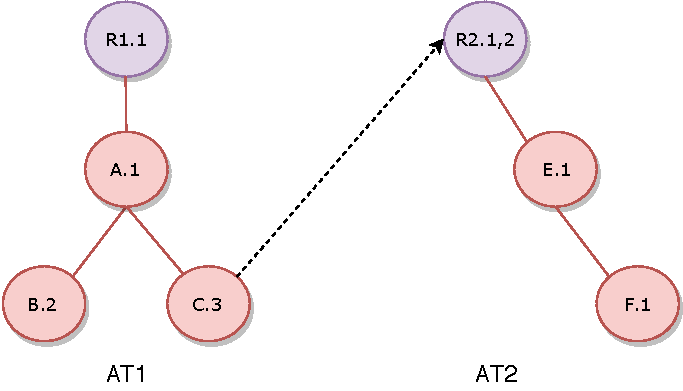
\includegraphics[width=3.0in,keepaspectratio]{obrazky-figures/alg_example1.pdf}\\[1pt]
	\caption{Stromy \textit{AT} a ich \textit{AN} uzly po spracovaní prvej vzorky dát.}
	\label{alg_example1_img}
\end{figure*} 

Stav \textit{AT} po spracovaní druhej vzorky dát zobrazuje diagram \ref{alg_example2_img}. Stav množín je v tabuľke \ref{alg_example2_tab} sa zmenil len pre množiny DataStore a Pattern. 
\begin{table}[hbt]
	\centering
	\label{alg_example2_tab}
	\begin{tabular}{|L{1.8cm}|p{12cm}|}
		\hline
		\textbf{Množina} & \textbf{Prvky} \\ \hline
		AT1 vzory & \(ATP1 = \{R1.1, A.1, B.2, C.3\}, ATP4 = \{R1.1, A.1, B.2, G.2\}\)\\ \hline
		AT2 vzory & \(ATP2 = \{R2.2\}, ATP3 = \{R2.1, E.1, F.2 \}\)\\ \hline		
		Pattern &\(CP1 = \{ATP1, ATP2, ATP3\}, CP2 = \{ATP4\} \)\\ \hline
		DataStore & 	\(B.2 = \{"ValueB", "ValueB2"\}, G.2 = \{"ValueG"\},\)\\
		 &  \(R2.2 = \{"ValueD"\}, F.2 = \{"ValueF"\}  \)   \\ \hline						
		
	\end{tabular}
	\caption{Tabuľka zobrazujúca stav množín po spracovaní druhého vzorku dát}
\end{table} 
\begin{figure*}[h]\centering
	\centering
	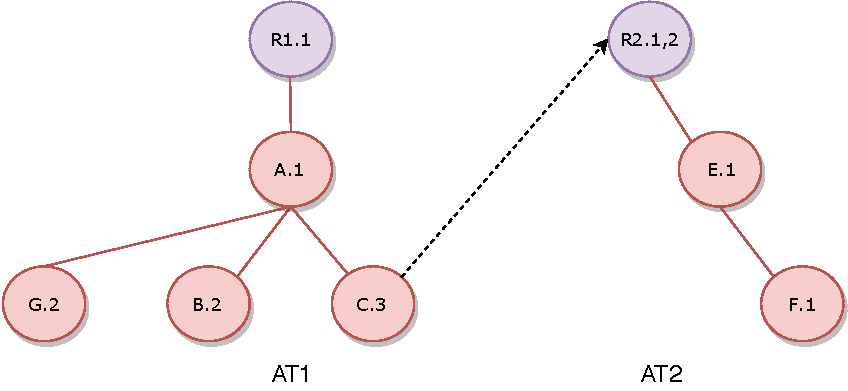
\includegraphics[width=4.0in,keepaspectratio]{obrazky-figures/alg_example2.pdf}\\[1pt]
	\caption{Stromy \textit{AT} a ich \textit{AN} uzly po spracovaní druhej a tretej vzorky dát.}
	\label{alg_example2_img}
\end{figure*} 
\caption{Diagram komponent nástroja TSD analyser spolu s nástrojmi Detector a Generator.}
Stav \textit{AT} po spracovaní tretej vzorky dát sa nezmenil, ostáva rovnaký ako v \ref{alg_example2_img}. Finálny stav množín je v tabuľke \ref{alg_example3_tab}. 
\begin{table}[hbt]
	\centering
	\label{alg_example3_tab}
	\begin{tabular}{|p{1.8cm}|p{12cm}|}
		\hline
		\textbf{Množina} & \textbf{Prvky} \\ \hline
		AT1 vzory & 	\(ATP1 = \{R1.1, A.1, B.2, C.3\}, ATP4 = \{R1.1, A.1, B.2, G.2\}\)   \\ \hline
		AT2 vzory & 	\(ATP2 = \{R2.2\}, ATP3 = \{R2.1, E.1, F.2 \}  \)   \\ \hline		
		Pattern &\(CP1 = \{ATP1, ATP2, ATP3\}, CP2 = \{ATP4\},\)\\ 
		& \(CP3 = \{ATP1, ATP2\}  \)\\ \hline
		DataStore & 	\(B.2 = \{"ValueB", "ValueB2", "ValueB"\}, G.2 = \{"ValueG"\},\)\\
		&  \(R2.2 = \{"ValueD", "VD", "VD"\}, F.2 = \{"ValueF"\}  \)   \\ \hline								
		
	\end{tabular}
	\caption{Tabuľka zobrazujúca stav množín po spracovaní tretieho vzorku dát}
\end{table} 
  
%\chapter{Implementácia nástroja tsd-detector}
\chapter{Záver}
\label{zaver}

V tejto práci boli najskôr predstavené princípy testovania založeného na dátach. Ďalej charakterizuje štrukturované dáta a ich formáty. Na základe analýzy požiadavok bol navrhnutý základ algoritmu pre automatizovanú detekciu závislostí vzoriek reálnych dát pre účely generovania testovacích dát, ktoré sú svojou štruktúrou a významom podobné reálnym vzorkám.  

Nasledovná práca spočíva vo vytvorení detailného návrhu a následnej implementácii nástroja, jeho otestovanie a integráciu v rámci Testos. 



%===============================================================================
